\chapter{Discussion}

This section details several of the design decisions that had to be taken regarding gameplay. It also discusses why other ideas were not implemented. The main goal was for the game to provide a new and fun experience for the user. This meant that a lot of effort was put into making the game exciting. This section also details some of the discussions that were held regarding the concept of the game. 

The discussion also provides some comments on how the project could have been managed better, and how certain issues could be handled more effectively.
%----------------------------------------------------------
\section{Design choices}

Deciding what features to implement was an important step in developing a foundation from which a marketable game could be developed. These decisions were based on evaluations of existing solutions already on the market, as well as some solutions that did not already exist on the market.
%----------------------------------------------------------
%----------------------------------------------------------
\subsection{Fixed path versus maze building}

The first important design decision that had to be taken included the movement pattern of the mobs. The Tower Defense genre is divided into two distinctive groups when it comes to mob movement over the map: fixed path and maze building. With a fixed path the mobs move along a pre-defined route on the track and towers can be built along its sides. Maze building games on the other hand, consist of an open field where mobs can move freely. It is up to the player to build obstacles forcing the mobs to take detours toward the exit. The obstacles that are used are in most cases the towers themselves. 

While testing different games during the research stage of development, one of the tested games was Robo Defense \citep{lupidLabs}, which featured maze-style gameplay. Robo Defense is a popular Tower Defense game with high rating on the Android market. Distinguishing Eskimo Tower Defense from this popular alternative was a big factor in deciding upon the fixed path design.

There are many benefits of using a fixed path model. Using a fixed path makes the game less complex to the player. It is more forgiving when it comes to the placement of towers: Maze building games can become frustrating if the control is imprecise, because a tower in the wrong place might destroy the entire maze. Another benefit is that it gives the level designer more control over the tracks, making it easier to vary track design by varying the path.

Another reason for using the fixed path solution was that none of the team members had much prior experience of game development. For this reason it was decided to keep the complexity at a minimum. The maze building solution would imply the use of artificial intelligence which would be too time consuming to implement, because of the increase in complexity. The static path design seemed to be the least complicated to use when developing a game for the first time. To assure a unique gameplay the focus was instead directed to other implementations, such as the snowball.
%----------------------------------------------------------
%----------------------------------------------------------
\subsection{Theme}

One of the major subjects of discussion in the group was the theme of the game. Since no one in the team had any experience of graphical programming, the theme was decided late in the project. At first, placeholders were used to test the functionality of the game. This was later changed to a temporary theme to get started with the graphics. 

It was decided that the game should have a background story that the theme should be linked to. In an early discussion, a green house effect-theme was discussed. The story would then be that animals from the north pole would flee from their melting environment. A map with that story would then have different themes, for instance polluting factories, melting ice caps and smog.

Finally it was decided to use an Eskimo theme. The background story was the same but instead of the green-house effect the animals were migrating south because they desired to move to a warmer climate. The Eskimo tribes frowns upon this since they depend on the wildlife for food and clothing. The tribes therefor set out to prevent this disaster from occurring. The maps will gradually become greener and warmer when progressing throughout the game. The towers were designed as different Eskimos, the snowman and the igloo canon. The mobs became animals such as penguins, polar bears and walruses. 
%----------------------------------------------------------
%----------------------------------------------------------
\subsection{Projectile algorithm}

During the discussion of how the projectiles should work, two different ways of implementing them were suggested. One way was to make them constantly follow their target, changing direction as they moved, like a homing missile. The other approach was to approximate where the mob and projectile would collide and aim in that direction. With this approach, the direction of the projectile does not change after being launched. 

Both methods where implemented to see which one had the best performance. It turned out that the homing missile method was optimal. Since the projectiles travel quite fast, most often reaching its target in about three frames, only three corrections of the angle were needed. When using the interception method the angle is only calculated once, however, this approach also requires the calculation of the future position of the mob. The code for the interception equation is shown in figure ~\ref{fig:codeEXInterception}.

%------
%- Code snippet intercepting projectile
%------
\begin{figure}[htb]

\begin{small}
\verbatiminput{code/interceptionCode.java}
\end{small}

\caption{Pseudo code for interception algorithm}
\label{fig:codeEXInterception}

\end{figure}
%------

The equation for the homing method is shown in figure ~\ref{fig:codeEXHoming}.

%------
%- Code snippet homing projectile
%------
\begin{figure}[htb]

\begin{small}
\verbatiminput{code/hoomingCode.java}
\end{small}

\caption{Pseudo code for homing algorithm}
\label{fig:codeEXHoming}

\end{figure}
%------

According to tests performed, the first equation is more than three times as resource-demanding as the second one. This can be explained by the use of Math.sin() and Math.asin() methods which are much more time demanding than a normal multiplying operation \citep{Green2}. It was therefore decided to use the homing missile method.

Another issue is how to detect a collision with a mob. Collision detection of a mob and a projectile is done by checking the distance between them. If the distance is smaller than a predefined value the objects are considered to have collided. The problem is which mob to calculate this for; either the target mob of the projectile or any mob coming in its way. The most intuitive approach would be the second one. The problem with this is that the projectile has to check for collision with all the mobs on the map. This can be very resource consuming, especially if there are a lot of mobs and projectiles currently on the map. It was therefore decided only to do collision detection for the target mob. The only real problem with this is that if a projectile misses its original target, it will not be able to hit another mob. Since we decided to use projectiles acting like homing missiles this would not be a problem.
%----------------------------------------------------------
%----------------------------------------------------------
\subsection{Waves}

A big issue was how the waves were supposed to work. In some Tower Defense games, such as Bloons \citep{bloons} and Flash Element Tower Defense \citep{elementTD}, the game pauses between every wave, giving the user time to build more towers. This means that the user will have to manually call the next wave. Another approach is to have the waves arrive continuously with a fixed amount of time between them. It was decided to use the delay approach. This was to ensure that the game would keep a steady pace and to remove unnecessary user actions. Since the tracks feature lot of waves this might be burdensome for the player to always have to press a button between each wave.

Since the mobs have varying speed, this may result in having one wave catch up with the previous wave. This is very noticeable during the boss waves. A boss wave consists of one mob with a lot more health than normal mobs, which means they take more effort to kill. Since there is only one mob in boss waves, the countdown for the next wave starts immediately after it has entered. To solve this, the delay after the boss waves was increased. 
%----------------------------------------------------------
%----------------------------------------------------------
\subsection{Unique features}
The development of the game called for distinguishing it from other Tower Defense games to make it more desirable for potential customers. Modern Android phones offer many new ways to control applications which could be taken advantage of. The idea was to add an extra dimension to the game using the phone's accelerometer. One of the ideas was to control the towers by tilting the phone. Another idea was that the player would be able to control the range of the towers. If the player would tilt the phone to the left, the towers' range would be increased in that direction. Another idea was to control the speed of the mobs. When tilting to the left, it would create a slope to the left making the mobs moving left go faster and mobs moving right go slower. 

The studies did not include any games that had multiple paths for the mobs. This would be an easy feature to implement that would make it more unique. Another thought was to allow the user to control which way the mobs walk in a crossroad using the accelerometer. The more the phone is tilted in one direction, the higher the probability is that the mobs choose that way.

The idea that eventually was implemented was the snowball. The snowball will roll over the map controlled by tilting the phone, almost like the classical board game Labyrinth. The player can use this snowball to kill mobs when in difficult situations. Some discussion was had regarding how the snowball would interact with the units on the map. Initially it was designed to kill every mob it touched. This was the easiest way to code it but it made the snowball too good, especially against bosses who had much more health than other mobs. Later, this was changed to dealing damage based on a percentage of the mobs health every frame it touched them. The snowball was also modified to deal less damage to bosses in order to make it less effective against them.

There was also a discussion whether the snowball should have any negative aspects to make it harder to use. One idea was to have the snowball not only damage the mobs but also the towers. This combined with a more powerful snowball would make it both effective in hard situations but also a risk. The problem with this is that the player then could place the snowball on the path and without tilting the phone kill mobs very effectively. This would discourage the user from tilting the phone, not using the snowball as it was intended. The snowball was well recieved in several of the post-development interviews. 

%----------------------------------------------------------
%----------------------------------------------------------
\subsection{User interface}

User interface is one of the most important areas when working with touchscreen mobile phones or small touchscreens in general. The small screen needs to hold a lot of information. Since the touchscreen is operated with the user's fingers, and some might have bigger fingers than others, it is important that items are not too small. This can make the player irritated when trying to touch the buttons. They should not be too big either because that would result in the game field being too small.

You want to fit as much information as possible on the screen, but you also want to keep it clean for the user. There were many discussions about which buttons would be the most important for the player during the different states of the game. To keep it clean, pressing a button often brings up a menu with several options to choose from.

The game is played with the screen in landscape position, meaning that most users will only use his thumbs to interact. This means that the buttons must be even bigger compared to if the index finger would have been used.
%----------------------------------------------------------
%----------------------------------------------------------
\subsection{Animations}

Animations were not the main priority during the development. At first, the development was focused on having a working game with innovative features. During testing, it became clear that a game with no animations would be pretty boring. To give the player a good experience the game needed a more realistic feeling. The interviews also revealed that sounds and animations were positive for the game experience. Therefor animations were added to the mobs, which made them look like they were wobbling back and forth when they were walking down the path. This small change made the game look much more dynamic. There is also an animation at the end of the path where the mobs dive into the water. 
%----------------------------------------------------------
%----------------------------------------------------------
\section{Game balance}

For a game to be interesting and thus sellable, it must provide just enough challenge to the user. In strategic games like Tower Defense, it is also important that there is room for different types of strategies. Both of these requirements are achieved by balancing the game. This section describes how the different parts of the game were balanced and why.

\subsection{Towers}

Balancing of the towers was done to make sure that no tower was superior to other towers. Being able to finish the game by only building one type of tower would make the game boring and unchallenging. The idea was that the player needed to build different towers for different situations. This is one of the reasons for having different types of towers and mobs. All maps contain different combinations of mob types, meaning the user has to change his strategy to meet the challenges he faces.
%----------------------------------------------------------
%----------------------------------------------------------
\subsection{Mob waves}

The biggest part of game balance included adjusting the characteristics of mob waves. Each mob awards the player with money when killed. Making the game balanced requires the income to be similar to the cost of building towers. If too much money was rewarded the game would not be challenging and if the reward was too small it would be impossible to finish the game.

Since the maps have different difficulties, we had to manually set the health of each mob wave. The waves of the first map should be easier than the waves of the second map, increasing the difficulty as the player progresses. 
%----------------------------------------------------------
\section{Critical project review}

At the end of the project, several points were raised that could have been approached in a different manner. The primary concern was that the developers gained a much greater understanding of the technology behind several of the key concepts. In particular, the way Android uses activities, but also the use of XML and how touch sensitivity was to be implemented. The project could have benefited from having these concepts studied and analysed further before work on implementation began. This would have meant that a greater understanding would have been gained which would have positively impacted the results, as well as increasing the efficiency of work done. 

The project would have progressed smoother if a more strict project development method was chosen and consistently followed. A discussion was held at the beginning of the project where the decision was made that a model of the project would be designed before implementation. This was to allow the team to focus on making many of the key design decisions early on, instead of having them come up at a later time disrupting work. This modelling prior to implementation was not fully completed, resulting in the same problems it sought to avoid. The amount of problems caused by poor design decisions might theoretically also have been greater because of this. 

One problem which could have been handled better was that of the cross platform functionality. Since several Android phones varied in screen size and resolution, we resorted to a compromise when drawing the canvas. This resulted in a slightly misplaced interface on certain phone models. This was handled by drawing a game field that was slightly larger than necessary, which resulted in the buttons being located in a less than optimal position on the larger phones compared to the smaller ones. This can be compared in figure XX.

%------------------------
%- Image of the game on desire and hero
%------------------------
\begin{figure}[here]

\begin{center}
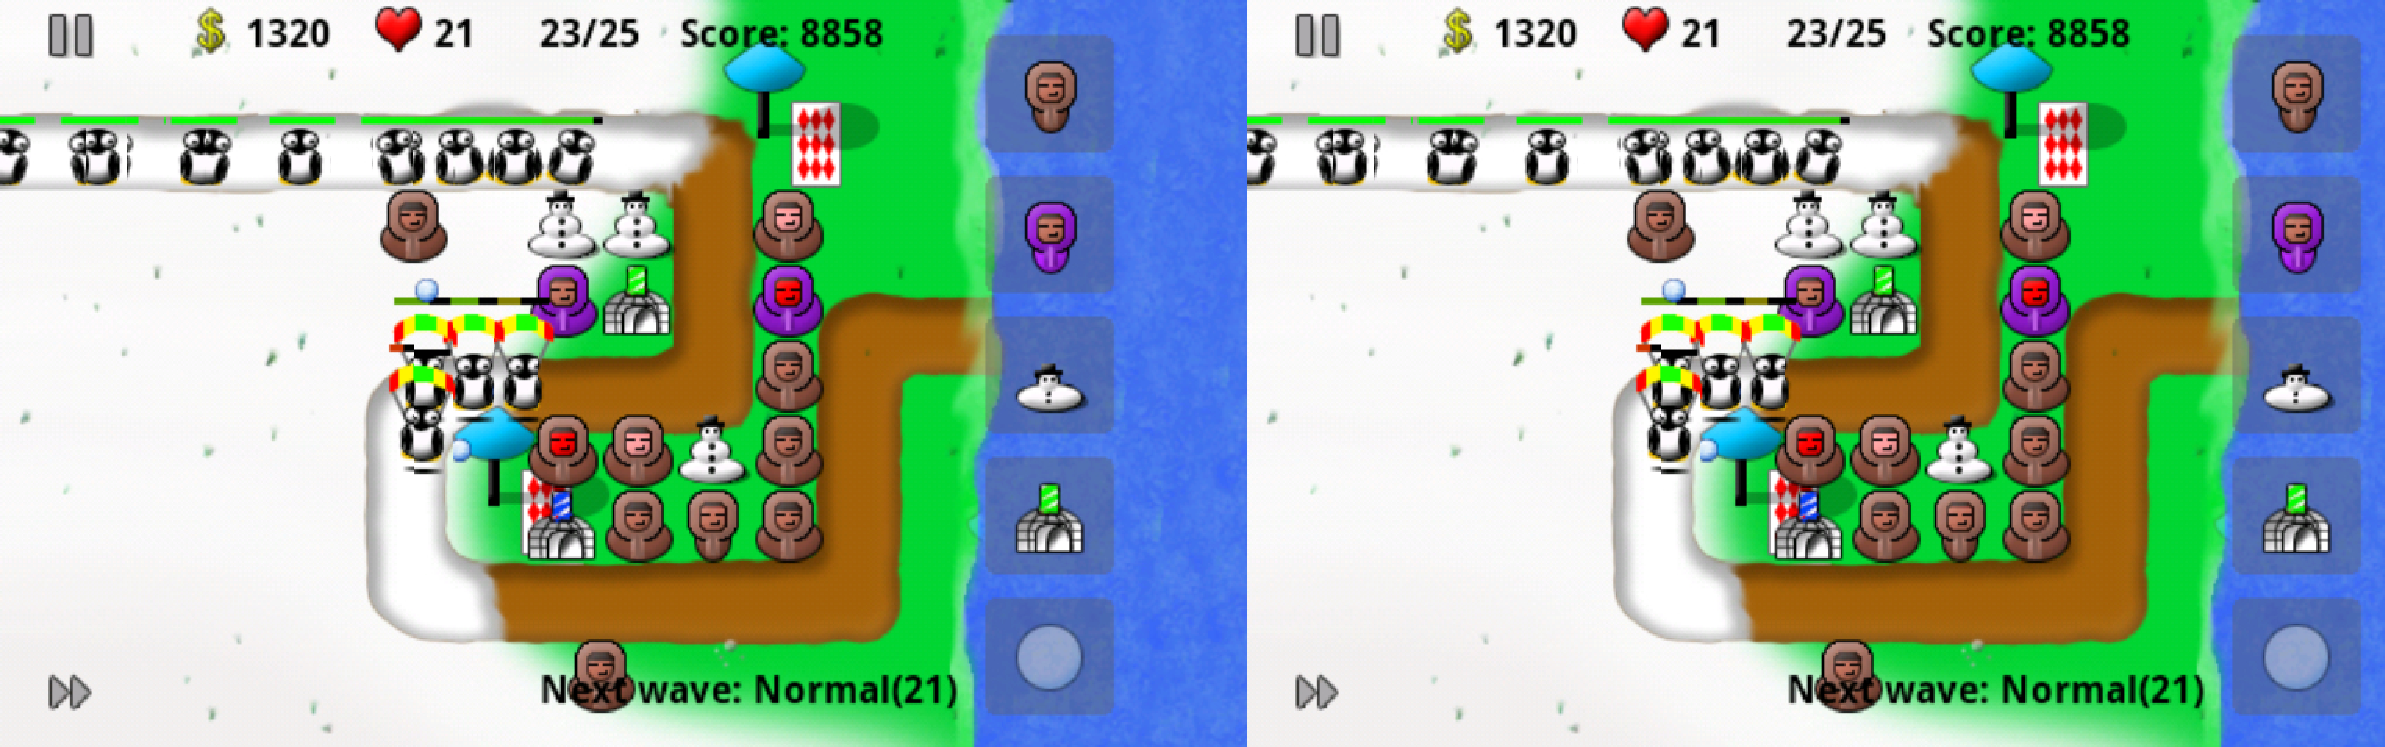
\includegraphics[scale=0.4]{pics/chapters/chapter5/frankingame}
\end{center}

\caption{To the left: The game on a HTC Desire, To the Right: The game on a HTC Hero}
\label{fig:desirehero}

\end{figure}
%------------------------
Several of the assumptions that ultimately decided many of the major design choices were somewhat based on results of the pre-development interviews. However, there are a few improvements that could have been made. The interviews were not in a particularly large scope, only detailing a few individuals, meaning that they likely do not represent a majority of the possible user base. The interviews were also conducted at a very early stage and failed to bring up several of the more important questions that were contemplated during the design discussions. Instead, the interviews were mostly focused on general questions which generated general answers without actually providing a base for several decisions. Design decisions were instead based on some of the most popular Tower Defense games.

A few interviews were also conducted after the development process to get a general idea of how players felt about certain aspects of the game. These interviews were mostly held with friends and family of the developers which might have heavily influenced their comments regarding the game. What the game might have needed was a more extensive pre-development and post-development research regarding the market, including focus groups, as well as further discussion. (Lindlof 2002) CITE
%----------------------------------------------------------
%----------------------------------------------------------
\section{Future work}

The game that resulted from this project is playable in its current state. However, additional features could be added to increase the value of the game. It is also an excellent basis from which a commercial game can be built. This chapter includes several implementations that were thought of but never realized.

\subsection{Public highscore}

To make the game more attractive and addictive, which was part of the purpose of the project, a public highscore could have been implemented. This would allow the users to play not only to complete the game, but also to compete against other players. A server would be needed to be able to upload and store the users' highscores. This was considered to take too much time and was not that important for the overall game experience, therefore it was not implemented.
%----------------------------------------------------------
%----------------------------------------------------------
\subsection{Cross-platform speed consistency}

If the game was ever to have a public highscore, the game would need to be fair. If the game runs faster on phones with more powerful processors it is not fair. In that case, players with slower phones would have an advantage compared to the rest of the players. To solve this the game has to run at the same speed independent of the speed of the phones' processors. There is also a problem with future phones that will have even more powerful processors. These phones would run the game so fast it would be very hard for users to play it. There are a number of well-known methods available to counter this effect. These were excluded from this project in favor of adding features that more directly affect the game experience. This issue has the highest priority of all future work.
%----------------------------------------------------------
%----------------------------------------------------------
\subsection{Sounds}

In the current version of the game the only sounds included are the background music and a sound effect played when the mobs reach the water. According to our last interviews many people wanted sound effects when mobs were killed. According to them, this would increase the addicting factors of the game. Implementing more sound effects was planned but there was no time to add this for all situations in the game.
%----------------------------------------------------------
%----------------------------------------------------------
\subsection{Achievments}

One thing that might increase the game's lifespan is the concept of achievements. This is a form of extra bonuses given to the player for completing various predetermined tasks. Completing these achievements would unlock new functionalities or new maps. These achievements could be relatively hard to complete. They would also give the user something to strive for after completing all the standard maps in the game. 
%----------------------------------------------------------
%----------------------------------------------------------
\subsection{Snowball improvement}

The snowball is one of the main parts that separates Eskimo Tower Defense from other Tower Defense games. To further improve the game experience, it is very important that this special weapon is fun and easy to use. If it is not implemented good enough, the player might not want to use it. He would then miss out on one of the things that makes the game unique. Further development of the snowball is therefore an important part to focus on.

Since the snowball is never introduced properly, new players might not notice that it exists. The snowball is one of the more unique parts of the game and it would be very bad if the player never uses it. A message or sound that indicates that the snowball is available would be helpful. The way the snowball is implemented could also be improved. It could for example bounce or even damage towers on the map to make it more challenging to use. The graphics for the snowball could also be improved. In the current version, the snowball is able to roll over the water. One suggestion was that is should sink or melt faster in the water. Instead of killing the mobs, there was an idea to have the snowball stun them. This would stop them from walking for a short moment, giving the towers more time to shoot them.
%----------------------------------------------------------
%----------------------------------------------------------
\subsection{Additional special weapons}

To make our game more unique, additional special weapons could be implemented. One idea was to variate the snowball with other player-controlled weapons. A weapon that would daze or stun the mobs momentary was discussed. This could be graphically represented as an earthquake for example. The idea of a meteor falling down from the sky was also discussed. These different weapons could be gained by completing different maps or achievements. They could also be available on certain maps where the special weapon is related to the theme of that map.
%----------------------------------------------------------
%----------------------------------------------------------
\section{Conclusion}

A Tower Defense game for Android has successfully been developed during this project. With regards to functionality, all of the major components that make up a Tower Defense game have been implemented, and would only require optimization to form the basis of a marketable game. Concerning the development of innovative game mechanics, the snowball was well recieved in the post-development studies and is a prime example of new user interaction features made possible on the Android platform. 

According to our post-development interview the balance of the game is a big part in the feeling of the game. After developing the game our conclusion is that the balancing is a very complicated part, that requires both time and insight into the game structure. When changing one type of balance variable it affects many other parts, requiring extensive testing before a complete game is produced.